\chapter{\label{ch:4}MWC modelling} 

\graphicspath{{figures/ch4/}}

\minitoc

\section{Modelling of ion channel function}

\subsection{Restricting the subset of possible models}

\subsection{Considerations for fitting a model}

\section{Implementing an MWC model}

\subsection{A simple case}

The simplest case of an allosteric MWC model for an ion channel is shown as Scheme I in Figure \ref{chxfig:mwc_model_diagrams}.
This simple case assumes a channel composed of a single monomer with a single binding site for ligand $A$.
The channel is restricted to two states, open and closed.
These two states exist in an equilibrium described by L, which is equivalent to $\frac{[open]}{[closed]}$.
Ligand $A$ binds to the protein with a microscopic affinity constant $K_A$.
The ligand $A$ differentially stabilises the open and closed states by a constant $D$.
When $D$ is unity, the ligand $A$ binds equally to both states and so does not influence the conformational changes of the channel.
When $D>1$, the ligand $A$ preferentially stabilises the open state, while when $D<1$ the ligand instead preferentially stabilises the closed state.

\begin{figure}[h]
	\centering
	\begin{subfigure}[t]{0.9\textwidth}
		\caption{}\label{chxfig:mwc_model_diagrams}
		\centering
		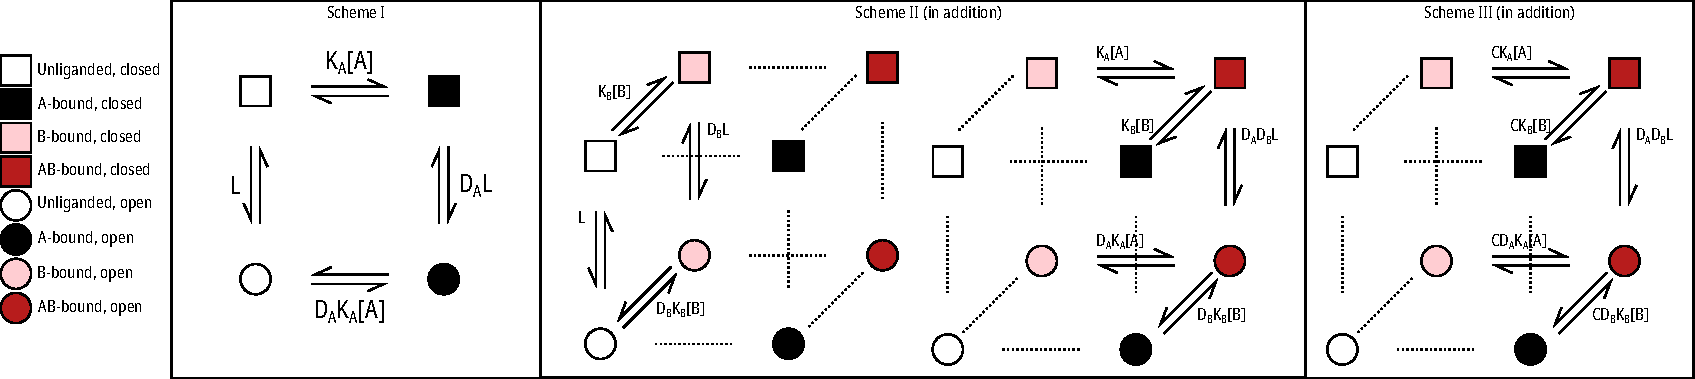
\includegraphics[width=\textwidth]{mwc_model_diagrams.pdf}
	\end{subfigure}
	\vfill
	\begin{subfigure}[t]{0.3\textwidth}
		\caption{}\label{chxfig:mwc_scheme_1_fits}
		\centering
		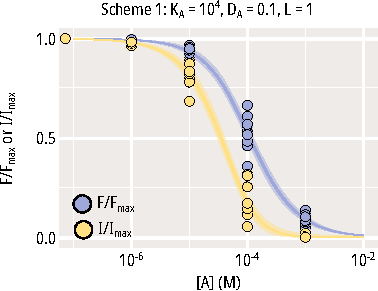
\includegraphics[width=\textwidth]{mwc_scheme_1_fits.pdf}
	\end{subfigure}
	\hfill
	\begin{subfigure}[t]{0.3\textwidth}
		\caption{}\label{chxfig:mwc_scheme_2_fits}
		\centering
		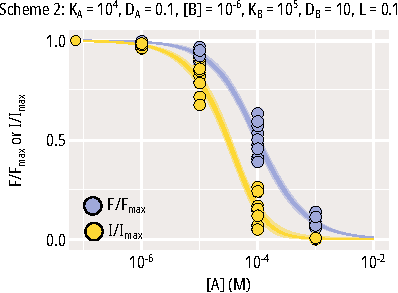
\includegraphics[width=\textwidth]{mwc_scheme_2_fits.pdf}
	\end{subfigure}
	\hfill
	\begin{subfigure}[t]{0.3\textwidth}
		\caption{}\label{chxfig:mwc_scheme_3_fits}
		\centering
		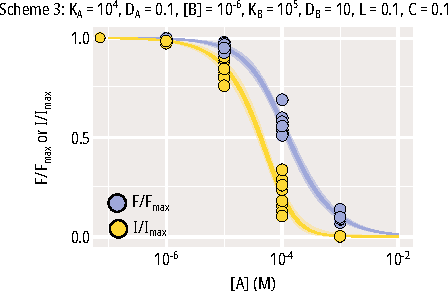
\includegraphics[width=\textwidth]{mwc_scheme_3_fits.pdf}
	\end{subfigure}
	\vfill
	\begin{subfigure}[t]{0.9\textwidth}
		\caption{}\label{chxfig:mwc_params_1}
		\centering
		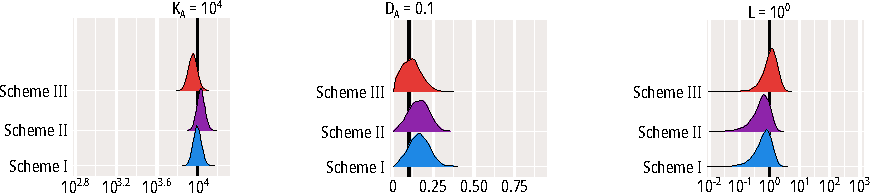
\includegraphics[width=\textwidth]{mwc_scheme_param_fits.pdf}
	\end{subfigure}
	\caption[Generating data from MWC model schemes]{
	\subref{chxfig:mwc_model_diagrams} Equilibrium diagrams for the three MWC schemes considered.
	For each scheme, only the parameters newly relevant for that scheme are shown explicitly.
	\subref{chxfig:mwc_scheme_1_fits}, \subref{chxfig:mwc_scheme_2_fits}, \subref{chxfig:mwc_scheme_3_fits} Data generated from Scheme I (\subref{chxfig:mwc_scheme_1_fits}), Scheme II (\subref{chxfig:mwc_scheme_2_fits}) or Scheme III (\subref{chxfig:mwc_scheme_3_fits}) all fit to Scheme I.
	The input parameters are shown above each panel.
	$L$ differs between \subref{chxfig:mwc_scheme_1_fits} and \subref{chxfig:mwc_scheme_2_fits}, \subref{chxfig:mwc_scheme_3_fits} due to the introduction of a resting PIP\textsubscript{2} concentration, which in Scheme I is implicitly incorporated into $L$.
	\subref{chxfig:mwc_params_1} Parameter estimates for the Scheme I model fit to the data generated by all three schemes.
	The input parameter value is marked as a black vertical line for each panel.
	}\label{chxfig:mwc_models}
\end{figure}

\subsection{The role of PIP\textsubscript{2}}

If we consider introducing a second ligand B which binds to a distinct site on the same monomer and does not directly interact with ligand A, we introduce the states shown in Scheme II of Figure \ref{chxfig:mwc_model_diagrams}.
Each ligand has its own microscopic association constant ($K_A$ or $K_B$) and its own preference for the open or closed states ($D_A$ or $D_B$).
Importantly, there is no interaction term between ligand $A$ and ligand $B$; the only way the binding of the ligands can impact each other is through effects on $L$.
Scheme II is therefore a restricted form of scheme III, which explicity introduces a term for local interaction ($C$) between binding sites for ligands $A$ and $B$ on the same monomer.
When $C$ is unity, Scheme III becomes Scheme II.
When $C<1$, binding of one ligand reduces the ability of the other ligand to bind on the same monomer.
When $C>1$, binding of one ligand enhances the ability of the other ligand to bind on the same monomer.

To study nucleotide binding to Kir6.2, I have used Scheme I (expanded to incorporate four identical monomers) as an approximation of the K\ATP{} channel, with ligand $A$ representing nucleotides.
To determine whether this approximation is appropriate, I generated data using each of the three schemes as the underlying model of channel function and then fit the generated observations to Scheme I (Figure \ref{chxfig:mwc_scheme_1_fits}, \ref{chxfig:mwc_scheme_2_fits}, \ref{chxfig:mwc_scheme_3_fits}).
Ten individual sets of observations were generated using the inputs shown above each figure panel as the centre of a lognormal distribution with a standard deviation of 0.25.
These observations were then fit to Scheme I (as done previously throughout the thesis) and the values of the three free parameters ($K_A$, $D_A$ and $L$) were estimated (Figure \ref{chxfig:mwc_params_1}).

\begin{figure}[h]
	\centering
	\begin{subfigure}[t]{0.3\textwidth}
		\caption{}\label{chxfig:scheme_1_ka_shift}
		\centering
		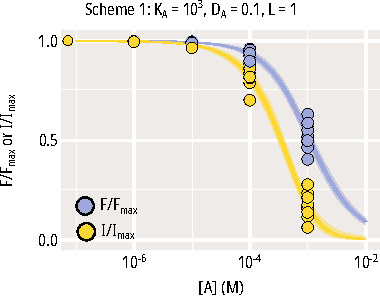
\includegraphics[width=\textwidth]{mwc_scheme_1_ka_shift.pdf}
	\end{subfigure}
	\hfill
	\begin{subfigure}[t]{0.3\textwidth}
		\caption{}\label{chxfig:scheme_1_da_shift}
		\centering
		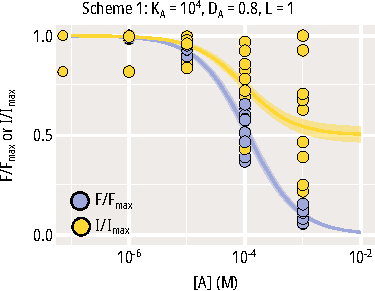
\includegraphics[width=\textwidth]{mwc_scheme_1_da_shift.pdf}
	\end{subfigure}
	\hfill
	\begin{subfigure}[t]{0.3\textwidth}
		\caption{}\label{chxfig:scheme_1_l_shift}
		\centering
		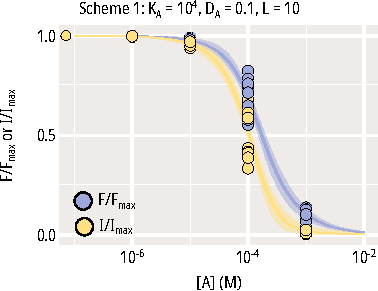
\includegraphics[width=\textwidth]{mwc_scheme_1_l_shift.pdf}
	\end{subfigure}
	\vfill
	\begin{subfigure}[t]{0.9\textwidth}
		\caption{}\label{chxfig:mwc_params_2}
		\centering
		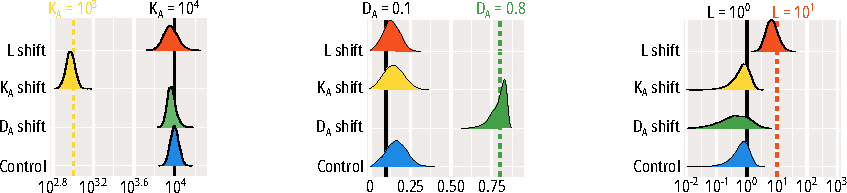
\includegraphics[width=\textwidth]{mwc_scheme_param_fits_2.pdf}
	\end{subfigure}
	\caption[Parameter retrieval from MWC models]{
	\subref{chxfig:scheme_1_ka_shift}, \subref{chxfig:scheme_1_da_shift}, \subref{chxfig:scheme_1_l_shift} Data generated from Scheme I with \subref{chxfig:scheme_1_ka_shift} $K_A$ shifted from $10^4$ to $10^3$, \subref{chxfig:scheme_1_da_shift} $D_A$ shifted from $0.1$ to $0.8$, or \subref{chxfig:scheme_1_l_shift} $L$ shifted from $1$ to $10$.
	\subref{chxfig:mwc_params_} Parameter estimates from each of the model fits.
	In each case, the modified parameter is retrieved accurately and no other parameters are affected.
	}\label{chxfig:scheme_1_shifts}
\end{figure}

We know that Scheme I is only an approximation of nucleotide binding as it does not explicitly include PIP\textsubscript{2}.
The question is, if the underlying data generating model is Scheme II which explicitly includes a second ligand, are we still able to extract meaningful parameter estimates by fitting the observed data to Scheme I?
In addition,to date it remains unclear whether there is local allostery between the nucleotide and PIP\textsubscript{2} binding sites.
The existence of local allostery would mean that Scheme III, which includes an explicit term for this interaction, would best represent the true data generating model.
We can show that even when Scheme II or Scheme III are the underlying data generating model, with ligand $B$ representing PIP\textsubscript{2}, we are still able to extract the true values of $K_A$ and $D_A$ by fitting the generated data to Scheme I (Figure \ref{chxfig:mwc_models}).
Parameter choices for Scheme II and III are such that the open probability of the channel at 0 [ATP] is still 50\%, equivalent to $L=1$ in Scheme I.
I really need to redo this with the true $L$ set to $0.01$ instead of $0.1$ as that is closer to post rundown open proability...

We can also show that when Scheme I is the underlying data generating model, changes in any of the three parameters are easily identified and retrieved by fitting the observed data to Scheme I (Figure \ref{chxfig:scheme_1_shifts}).
This suggests that introducing mutations which directly effect any of the three parameters of this model would be easily identifiable if Scheme I was the true underlying model.

What if Scheme II or III were the underlying model?
We would still expect changes in the three parameters which exist in Scheme I to be identifiable (I should probably check this), although $L$ would not represent the true unliganded open/closed equilibrium as we would be estimating an $L$ modified by the resting PIP\textsubscript{2} concentration, $K_B$, $D_B$ and $C$ - in this case, the estimated $L$ parameter in fact represents the ATP-unbound open/closed equilibrium.

\begin{figure}[h]
	\centering
	\begin{subfigure}[t]{0.45\textwidth}
		\caption{}\label{chxfig:scheme_2_kb_shift}
		\centering
		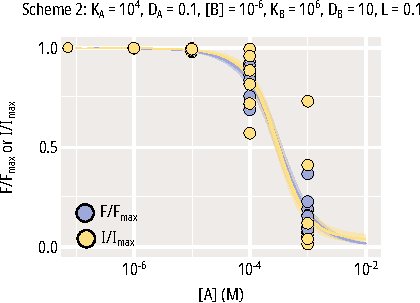
\includegraphics[width=\textwidth]{mwc_scheme_2_kb_shift.pdf}
	\end{subfigure}
	\hfill
	\begin{subfigure}[t]{0.45\textwidth}
		\caption{}\label{chxfig:scheme_3_kb_shift}
		\centering
		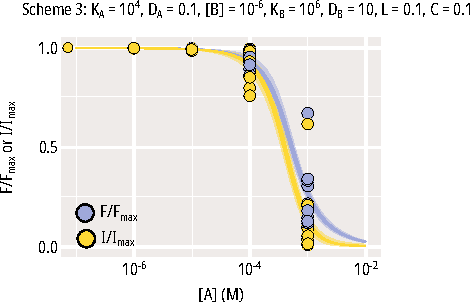
\includegraphics[width=\textwidth]{mwc_scheme_3_kb_shift.pdf}
	\end{subfigure}
	\vfill
	\begin{subfigure}[t]{0.9\textwidth}
		\caption{}\label{chxfig:mwc_params_3}
		\centering
		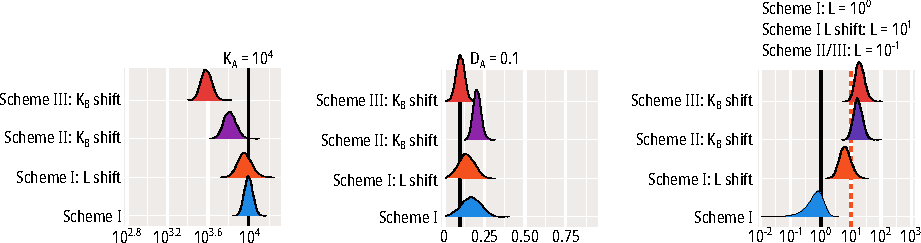
\includegraphics[width=\textwidth]{mwc_scheme_param_fits_3.pdf}
	\end{subfigure}
	\caption[Parameter retrieval from MWC models]{
	\subref{chxfig:scheme_2_kb_shift}, \subref{chxfig:scheme_3_kb_shift} Data generated from \subref{chxfig:scheme_2_kb_shift} Scheme II  or \subref{chxfig:scheme_3_kb_shift} with $K_B$ shifted from $10^5$ to $10^6$.
	}\label{chxfig:scheme_2_3_shifts}
\end{figure}

However, it is unclear how changes in parameters which are not explicitly modelled in Scheme I will affect the generated data and the parameter estimates obtained by fitting the data to Scheme I.
Figure \ref{chxfig:scheme_2_3_shifts} shows the results of increasing $K_B$ by tenfold on data generated from Scheme II (Figure \ref{chxfig:scheme_2_kb_shift}) or Scheme III (Figure \ref{chxfig:scheme_3_kb_shift}).
The first observation of note is that the generated data closely resemble those generated from Scheme I when $L$ is increased (Figure \ref{chxfig:scheme_1_l_shift}), and indeed when the $L$ parameter estimates for a tenfold shift in $K_B$ in Scheme II/III and tenfold shift in $L$ for Scheme I are compared (Figure \ref{chxfig:mwc_params_3}, right panel) are compared they appear to be similar.
So far so good, as an observed increase in $L$ when fit with Scheme I would lead us to draw the correct inferences about changes in the underlying model (i.e. the open probability of the cnall has indeed increased).
However, changes in $K_B$ are not perfectly captured by changes in $L$ when fit to scheme I.
Notably, if local allostery exists between the nucleotide and PIP\textsubscript{2} binding site - if Scheme III is the true underlying model - then fitting the observed data to Scheme I would lead us to estimate an incorrect value for $K_A$ (Figure \ref{chxfig:scheme_2_kb_shift}).
Thus, if there is local allostery between the sites, then a mutation which induces an increase in the binding affinity for PIP\textsubscript{2} would not just increase our estimate of $L$ (which would lead to a correct inference) but it would also decrease our estimate of $K_A$ by a not-insignificant amount, which could lead to the incorrect inference that a mutation is causing a direct change in nucleotide binding when it is in fact causing a direct change in PIP\textsubscript{2} binding, which through local allostery is influencing our estimates of $K_A$.
